% ============================================================
%  Chapter 2 — Related Work
% ============================================================
\chapter{Related Work}
\label{ch:related}

\myquotation{%
The history of science is the history of struggles against the default assumption.}{%
Anonymous}

This chapter reviews prior work that is relevant to the approach taken in this
thesis.
We cover classical and learning-based IID methods in Sections \ref{sec:classical_iid}
and \ref{sec:learning_iid}, work on multi-illuminant scenes and colour constancy in
\secref{sec:multiillum}, and the evaluation benchmarks we use in \secref{sec:benchmarks}.


\section{Classical Intrinsic Image Decomposition}
\label{sec:classical_iid}

The problem of separating illumination from reflectance is rooted in Retinex
theory \mycite{land71retinex}. Its starting observation is that perceived
lightness depends strongly on spatial comparisons, not only on the number
recorded at one pixel. If neighbouring image intensities are $I_1=A_1S_1$ and
$I_2=A_2S_2$, their ratio is
\begin{equation}
  \frac{I_1}{I_2}=\frac{A_1}{A_2}\frac{S_1}{S_2}.
  \label{eq:retinex_ratio}
\end{equation}
When illumination varies slowly over that small neighbourhood,
$S_1/S_2\approx1$, so the observed ratio is evidence for a reflectance change.
For example, a painted black stripe on a white wall should remain a material
boundary as the room becomes brighter. A soft illumination gradient should not.
Retinex-style methods classify or threshold such local changes and propagate the
surviving ratios to estimate a reflectance field.

This is foundational because it turns an impossible per-pixel factorisation into
a problem that can use spatial context. It is also only a prior. A hard cast
shadow can change abruptly and resemble paint; textured material can vary rapidly;
specular highlights violate the diffuse product model. The common shorthand
``illumination is low-frequency and reflectance is high-frequency'' is therefore
a useful intuition, not a physical rule. Modern learned methods replace many
hand-designed thresholds with data, but they still rely on the same distinction
between material changes and lighting changes.

\figref{fig:retinex_ambiguity} shows why such assumptions are necessary. Even a
simple brightness gradient has multiple exact decompositions: the image alone
does not reveal whether the change came from the surface or the light.
\begin{figure}[t!]
  \centering
  \resizebox{\textwidth}{!}{%
  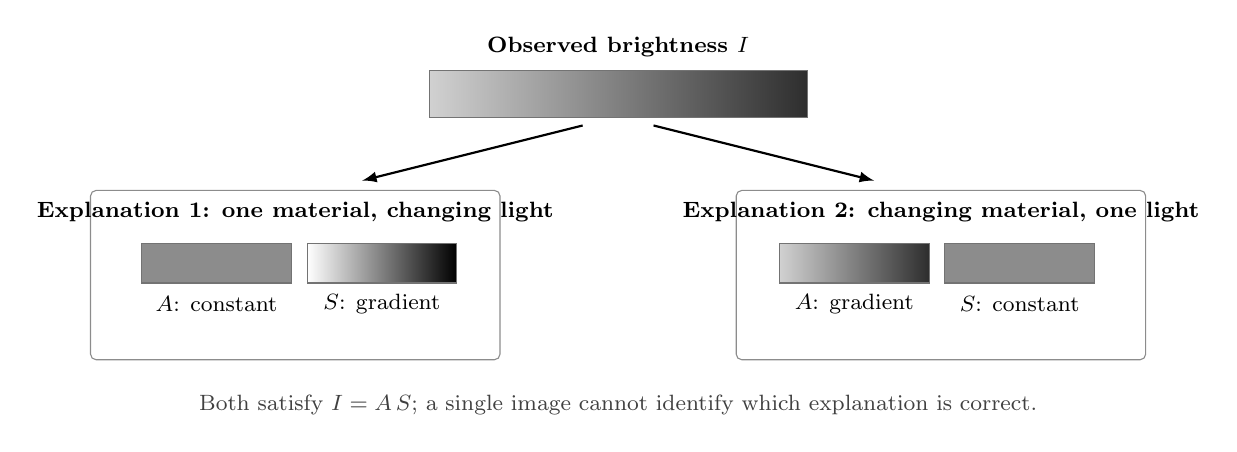
\begin{tikzpicture}[
    font=\small,
    >=latex,
    box/.style={draw=black!45, rounded corners=2pt, inner sep=7pt},
    lab/.style={font=\footnotesize\bfseries, align=center}
  ]
    \node[lab] at (0,1.55) {Observed brightness $I$};
    \shade[left color=black!18,right color=black!82,draw=black!55]
      (-2.4,0.65) rectangle (2.4,1.25);

    \node[box, minimum width=5.2cm, minimum height=2.15cm] at (-4.1,-1.35) {};
    \node[lab] at (-4.1,-0.55) {Explanation 1: one material, changing light};
    \fill[black!45,draw=black!55] (-6.05,-1.45) rectangle (-4.15,-0.95);
    \shade[left color=white,right color=black,draw=black!55]
      (-3.95,-1.45) rectangle (-2.05,-0.95);
    \node[font=\footnotesize] at (-5.1,-1.72) {$A$: constant};
    \node[font=\footnotesize] at (-3.0,-1.72) {$S$: gradient};

    \node[box, minimum width=5.2cm, minimum height=2.15cm] at (4.1,-1.35) {};
    \node[lab] at (4.1,-0.55) {Explanation 2: changing material, one light};
    \shade[left color=black!18,right color=black!82,draw=black!55]
      (2.05,-1.45) rectangle (3.95,-0.95);
    \fill[black!45,draw=black!55] (4.15,-1.45) rectangle (6.05,-0.95);
    \node[font=\footnotesize] at (3.0,-1.72) {$A$: gradient};
    \node[font=\footnotesize] at (5.1,-1.72) {$S$: constant};

    \draw[->,thick] (-0.45,0.55) -- (-3.25,-0.15);
    \draw[->,thick] (0.45,0.55) -- (3.25,-0.15);
    \node[font=\footnotesize,align=center,text=black!75] at (0,-3.0)
      {Both satisfy $I=A\,S$; a single image cannot identify which explanation is correct.};
  \end{tikzpicture}
  }
  \caption[Why intrinsic decomposition is ambiguous.]{%
    The intrinsic-image ambiguity in one dimension. The same observed brightness
    gradient can be explained by constant reflectance under changing illumination
    (left), or by changing reflectance under constant illumination (right).
    Retinex and learned IID methods resolve this underdetermined factorisation by
    adding spatial, semantic, and data-derived priors.
  }
  \label{fig:retinex_ambiguity}
\end{figure}


\mycitetext{grosse09mit} introduced the MIT Intrinsic Images dataset,
the first public benchmark for IID, and used it to show that simple Retinex
baselines outperformed more sophisticated methods of the time on real photographs.
A consistent finding from this benchmark is that the problem is extremely
ill-posed: many different (albedo, shading) pairs explain the same image.
Without strong priors, models tend to find trivial solutions.

The most influential approach to adding structure to the ill-posed problem is
Shape, Illumination, and Reflectance from Shading (SIRFS) by
\mycitetext{barron15sirfs}.
SIRFS frames IID as an energy minimisation over albedo, shading, and surface
normals jointly.
It encodes strong priors: albedos should be piecewise-constant, shadings should be
smooth, and surface normals should form a plausible scene geometry.
SIRFS significantly outperformed previous methods and remained a strong baseline
for several years.
However, its hand-designed priors struggle on complex real-world scenes with
cluttered backgrounds, unusual lighting, or materials that violate the
piecewise-constant albedo assumption.


\section{Learning-Based Intrinsic Image Decomposition}
\label{sec:learning_iid}

The availability of large synthetic datasets shifted the field toward learned models.
\mycitetext{li18cgintrinsics} proposed CGIntrinsics, a set of physically-based
re-renderings of synthetic indoor scenes that provides paired
(image, albedo, shading) training data at scale.
They showed that a CNN trained on this data, combined with ordinal supervision
from the human judgements of IIW \mycite{bell14iiw}, generalises well to real
photographs.
CGIntrinsics established the pattern that has dominated the field since:
train on photorealistic synthetic data with ground-truth labels, then evaluate
on real images.

\mycitetext{bell14iiw} introduced the Intrinsic Images in the Wild (IIW) benchmark,
which takes a different approach to ground truth.
Rather than rendering or measuring true albedos, IIW collects human judgements about
relative albedo comparisons: for any two surface patches in a photograph, human
annotators say which one is lighter.
This produces a set of relative constraints that any valid albedo prediction must
satisfy.
The evaluation metric, the Weighted Human Disagreement Rate (WHDR), measures how
often the model's albedo ordering disagrees with the majority of human annotators.
IIW became the standard benchmark for IID for many years and is still widely used.
Its limitation is that it captures perceptual shading quality (whether shadows look
right) more than it captures the accuracy of the recovered material colour.

A line of work by Careaga and Aksoy is the closest to ours in its treatment of
illumination colour.
Ordinal Shading \mycite{careaga23ordinal} decomposes real photographs by first
estimating shading up to an ordinal (ordering) constraint, which is far more
robust than absolute regression, and then refining the albedo; its shading is
still greyscale.
Its successor, Colorful Diffuse IID (CD-IID) \mycite{careaga24cdiid}, is the
first method to explicitly predict a \emph{colored} diffuse shading in the wild,
through a multi-stage cascade (grey decomposition, then a low-resolution
chromaticity network, then albedo and diffuse-shading refinement) and an analytic
non-diffuse residual.
CD-IID is the direct point of comparison for the goal of this thesis: it shows
that colored shading is representable, but its training never \emph{constrains}
the albedo to be invariant across illuminant changes. Consequently, the colour split between
albedo and shading is learned only implicitly from single images.
Our work adds exactly that missing constraint, using real cross-illuminant pairs.

In parallel, diffusion-based models have become strong IID baselines.
Marigold-IID \mycite{marigoldiid24} fine-tunes a Stable-Diffusion backbone for
IID and ships two variants: an \emph{appearance} model trained on InteriorVerse
that targets material properties (albedo, roughness, metallic), and a
\emph{lighting} model trained on Hypersim \mycite{roberts21hypersim} that targets
albedo, diffuse shading, and a non-diffuse residual.
Both produce visually sharp decompositions and excellent zero-shot WHDR on IIW.
We use Marigold-IID as our primary experimental baseline because checkpoints are
public, its lighting variant shares our model's training distribution (Hypersim), and
it represents the current generative state of the art.
Very recent work reaches for external knowledge instead: ReasonX
\mycite{reasonx25} guides the decomposition with a multimodal language model and
reports strong IIW WHDR improvements; no public checkpoint was available at the
time of writing, so we cite its published numbers only where protocols match.

\paragraph{Comparison scope.}
The methods above are not all compared in the same way. We run models locally
only when an official checkpoint and compatible output are available: Marigold-IID,
CRefNet, and Ordinal Shading. We cite CD-IID, ReasonX, and older methods from
their papers only when the dataset split and metric match our protocol. This
distinction matters because a published number obtained with different training
data, resizing, or test scenes is context, not a controlled head-to-head result.
Chapter~5 marks locally reproduced and literature-cited rows separately and
explains why each model is included.

The fundamental limitation shared by these methods is that none of them
explicitly \emph{supervises} the separation of illuminant colour from material
colour.
When the scene is lit by a coloured light, the illuminant hue can bleed into the
predicted albedo, because nothing in the training objective says it should not.
Our work addresses this gap with a constraint mined from multi-illuminant data.


\section{Multi-Illuminant Scenes and Colour Constancy}
\label{sec:multiillum}

The specific challenge of coloured illumination in IID has received relatively
little attention compared to the broader IID problem.
Most methods implicitly assume a single white or near-white illuminant.

The cost of that assumption is arithmetic rather than model-specific. If shading
is scalar, it has no hue, so a coloured illuminant must be represented in the
only RGB factor: albedo. Chapter~3 derives this limitation and demonstrates it
visually in \figref{fig:formulation}; this section focuses on how prior work has
responded to it.

Work on multi-illuminant colour constancy in computational photography provides
useful context.
\mycitetext{beigpour13miid} addressed the problem of estimating multiple coloured
illuminants from a single image using a conditional random field formulation.
They created the MIID dataset, which contains scenes photographed under combinations
of coloured light sources with ground-truth illuminant annotations.
This is a different task from IID (they estimate illuminant colours rather than
separate albedo from shading), but the setup is closely related and provides
inspiration for the multi-illuminant pair training we use in this work.

The closest prior work to the constraint we propose is the self-supervised
decomposition network of \mycitetext{kinoshita21consistency}.
They observe the same gap we do: most IID methods do not enforce any consistency
on the \emph{reflectance} layer, and the usual white-illuminant model cannot
express a coloured light in the first place.
Their answer is to adopt a colour-illuminant model and to train with losses
computed over several illumination conditions of the same content, so that the
predicted reflectance is pushed to agree across them.
The difference from our work lies in where those conditions come from.
Their illumination variants are \emph{simulated}, which makes the supervision
cheap but ties it to the realism of the simulator.
We instead mine the constraint from real photographs of real rooms under real
bounced light (\secref{sec:mid_dataset}), where the illuminant chromaticity
varies for physical reasons rather than by construction.
The measurements in \chapref{ch:experiments} show why this distinction matters:
a synthetic tint applied to an image is not distributed like a real illuminant,
and training on the synthetic version measurably hurt constancy.

This family of work also suggests the shape of a sensible metric.
If a model is genuinely illuminant-invariant, the chromaticity it assigns to one
physical material must not move when the light changes.
Our constancy measures ($C_{\text{mat}}$ on MID, $C_{\text{arap}}$ and
$\text{Cast}_{\text{RMS}}$ on ARAP) are built directly on that statement: they
group the renderings or photographs of one scene by illuminant condition and
report how much the predicted albedo drifts across the group
(\secref{sec:mid_results}).
They are internal diagnostics rather than a published protocol, which is why we
report them alongside, not instead of, the measured-albedo benchmarks.


\section{Evaluation Benchmarks}
\label{sec:benchmarks}

We evaluate our model on four benchmarks that together cover different aspects of IID
quality.

\paragraph{Dataset, split, protocol, and benchmark.}
These terms are kept distinct throughout the thesis. A \emph{dataset} is a
collection of images and annotations. A \emph{split} identifies which samples
are used for training, validation, or testing. An evaluation \emph{protocol}
specifies preprocessing, eligible samples, and a metric. A \emph{benchmark} is
the held-out data together with that protocol. Thus MID is both a source of
training pairs and an evaluation dataset, but the CARI training scenes and the
30-scene test split never overlap. Calling a collection a ``database'' adds no
useful distinction here, so this thesis uses \emph{dataset} consistently.

The four benchmarks answer different questions. MID tests whether a real
surface stays stable across lights; MAW measures real material colour on sampled
regions; ARAP provides dense synthetic albedo and repeated illumination; IIW
tests whether predicted relative reflectance agrees with people. No single score
is treated as a complete definition of IID quality.

\subsection{IIW}

Intrinsic Images in the Wild \mycite{bell14iiw} is the most widely used benchmark
in the IID literature.
It contains 5,230 real indoor and outdoor photographs collected from the internet,
annotated with human pairwise reflectance comparisons.
The evaluation metric is WHDR: the fraction of annotator pairs (weighted by
confidence) with which the model's albedo ordering disagrees.
Lower WHDR is better.
IIW rewards agreement with perceived relative reflectance. Its human labels are
appropriate for that perceptual question, but the ordinal lightness comparison
does not measure RGB colour, absolute albedo, or dense texture.
We evaluate on the standard test split of 1,046 images (every fifth image of the
5,230), and report WHDR as the mean over images rather than pooled over
judgements.

\subsection{MID: Multi-Illuminant Dataset}
\label{sec:mid_dataset}

MID, the Multi-Illumination Dataset of \mycitetext{midintrinsics}, is the dataset
most directly relevant to the goal of this work.
It contains over 1{,}000 real indoor scenes, each photographed 25 times from a
fixed viewpoint with a flash bounced in a different direction for every shot.
Because the bounced light picks up the colour of the wall or ceiling it reflects
from, the \emph{effective illuminant chromaticity varies across the 25 conditions}
(we measured a 15--25\% chromaticity spread on the dataset's mirror-probe
annotations), while the scene and camera stay pixel-aligned.
The key property is that the true albedo of each surface does not change across
the illuminant conditions; only the illuminant does.
This makes it possible to define a constancy metric ($C_{\text{mat}}$) that measures
how much the scale-normalised predicted albedo lightness changes across conditions.
A model with perfect illuminant invariance would achieve $C_{\text{mat}} = 0$.
We hold out 30 scenes as a test split and report constancy on those; the training
split is used for the CARI pairs (\chapref{ch:implementation}).

\subsection{ARAP}
\label{sec:arap_dataset}

ARAP (``As Real As Possible'') is a synthetic high-dynamic-range dataset of
around 50 rendered indoor and outdoor scenes \mycite{arap}.
A subset of scenes ships with multiple renderings under different lighting
conditions (direction, intensity, and in some scenes light colour); we evaluate
constancy on the 37 multi-light scene groups (23 indoor), and additionally
report the coloured-illuminant subset in which the light \emph{colour} varies
across renderings, which is the axis this thesis targets.
ARAP provides ground-truth albedo images, which allows measuring not only constancy
across conditions (the $C_{\text{arap}}$ and $\text{Cast}_{\text{RMS}}$ metrics)
but also the accuracy of the predicted albedo against the ground truth.
The constancy metrics group scene renderings by the illuminant condition and
measure how consistent the predicted albedo is across groups.
Our local study reports LMSE, SSIM, and a mean-normalised RMSE diagnostic. This
implementation is not the least-squares scale-invariant RMSE used in published
ARAP tables, so Chapter~5 keeps the local and published protocols separate.
The two types of metric capture different things: a model can have good constancy
(stable albedo across illuminants) while still being wrong about the absolute
material colour, and vice versa.

\subsection{MAW: Measured Albedo in the Wild}
\label{sec:maw_dataset}

MAW \mycite{maw} is a benchmark of real indoor images paired with ground-truth
albedo measurements obtained through a controlled physical measurement process.
It provides a direct measure of albedo colour accuracy through two metrics:
$\Delta E$ (the CIELAB colour difference between predicted and measured albedo)
and intensity SI-MSE (scale-invariant mean square error on the luminance channel).
$\Delta E$ captures colour error in a perceptually motivated space after the
official scorer's per-material scale alignment.
MAW is particularly valuable because it measures real scenes where the illuminant
colour is part of the challenge, making it complementary to the synthetic ARAP.
We evaluate on 874 images from the MAW test split.
